\documentclass[letterpaper,11pt, spanish]{article}

%acentos de la forma ´ en vez de \'a
\usepackage[utf8]{inputenc}
\usepackage{babel}
\makeatletter

\usepackage[letterpaper]{geometry}

\usepackage{hyperref}
\usepackage{graphicx}
\usepackage{setspace}
\usepackage{color}
\usepackage{hyperref}
\usepackage{amssymb}
\usepackage{url}
%\usepackage{pdfpages}
\usepackage{fancyhdr}
\usepackage{hyperref}
\usepackage{amsmath}
\usepackage{amsthm}
\usepackage{booktabs}
\usepackage{subfig}
\usepackage{tikz}
\usetikzlibrary{arrows,automata}
\usepackage{listings} %Codigo
\lstset{language=C, tabsize=4,framexleftmargin=5mm,breaklines=true}
\newenvironment{enumerate2}{
\begin{enumerate}
	\setlength{\itemsep}{0pt}
	\setlength{\parskip}{0pt}}{
\end{enumerate}
}

\begin{document}
\onehalfspace{}

%\begin{sf}

% --------------- ---------PORTADA --------------------------------------------
\newpage
\pagestyle{fancy}
\fancyhf{}
%-------------------- CABECERA ---------------------
\fancyhead[L]{Universidad de Chile \\ Facultad de Cs. Físicas y Matemáticas \\ Departamento de Ciencias de la Computación \\ CC5113 - 1}
\fancyhead[R]{
\includegraphics[scale=0.3]{LogoUIngenieria.png}}
%------------------ TÍTULO -----------------------
\vspace*{6cm}
\begin{center}
\Huge  {Aprendizaje Automático Bayesiano}\\
\vspace{1cm}
\huge {Definición de Proyecto} \\
\end{center}
%----------------- NOMBRES ------------------------
\vfill
\begin{flushright}
\begin{tabular}{ll}
& Autores: Vicente Oyanedel \\
& 			Francisco Clavero \\
& Profesor: Pablo Guerrero \\
& \today \\
& Santiago, Chile.
\end{tabular}
\end{flushright}

% ·············· ENCABEZADO - PIE DE PAGINA ············
\newpage
\pagestyle{fancy}
\fancyhf{}

%Encabezado
%\fancyhead[L]{\rightmark}
\fancyhead[L]{\small \rm \textit{Sección \rightmark}} %Izquierda


\fancyfoot[L]{\small \rm \textit{CC5113 - Vicente Oyanedel, Francisco Clavero}} %Izquierda
\fancyfoot[R]{\small \rm \textit{\thepage}} %Derecha
%\fancyfoot[C]{\thepage} %Centro

\renewcommand{\sectionmark}[1]{\markright{\thesection.\ #1}}
\renewcommand{\headrulewidth}{0.5pt}
\renewcommand{\footrulewidth}{0.5pt}

% =============== INDICE ===============

\tableofcontents

% =============== BLOQUE DECODIFICADOR ===============
\newpage
\section{Descripción Detallada del Proyecto}

\href{las.leagueoflegends.com}{League of Legends} es un videojuego del estilo MOBA (Multiplayer Online Battle Arena),
donde dos equipos de 5 jugadores se enfrentan en una lucha por destruir el nexo
(base) enemigo. \\

\begin{figure}[h]
	\begin{center}
		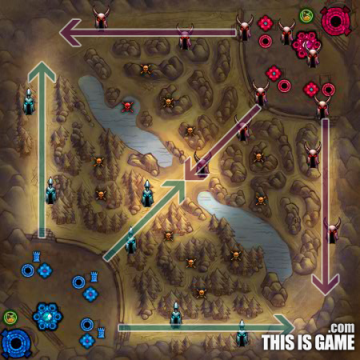
\includegraphics[scale=0.75]{map.png}
	\end{center}
	\caption{Mapa con los objetivos del juego.}
\end{figure}

Durante una partida, cada jugador puede controlar uno de aproximadamente 150 campeones
distintos. Cada uno tiene distintas habilidades y atributos, que determinan
su forma de uso, dificultad y proposito dentro del juego. Esto provoca que
los campeones sean muy distintos entre si, y que cada jugador tenga una afinidad
distinta por cada campeón, sea por gusto o por su rendimiento con ellos. La simplicidad
de los objetivos y a variedad de los campeones hace a League of Legends un juego
muy dinámico, a lo cual debe su fama. \\

Cada jugador tiene una cuenta de usuario con la cual se autentifica para jugar, y
almacena estadistidísticas de cada partida jugada. Esto incluye datos como
la cantidad de partidas jugadas, ganadas, o perdidas, la cantidad de contrincantes vencidos,
los campeones que ha usado, entre otros, con las cuales se puede caracterizar a
los usuarios. \\

El proyecto consiste en crear un sistema que recomiende campeones a un usuario de
League of Legends con los cuales pueda tener un buen rendimiento en el juego,
basado en las características de dicho usuario. \\

La recomendación se realiza en base a los campeones que utilizan usuarios con
características similares a las del usuario que ingresa al sistema. Para lograr
identificar los distintos grupos de jugadores similares, se utilizarán técnicas
de clustering. \\

Una vez terminado el \textit{Clustering} se generan 5 rankings a modo de recomendaciones de campeones, generadas en base a los jugadores del cluster del usuario. Estos 5 rankings corresponden a distintas recomendaciones que son explicadas a continuación:

\subsection{Collaborative Filtering}
Cada usuario de League of Legends puede jugar con 127 campeones distintos. Al jugar una partida un jugador gana \textit{Champion Points} con \textbf{el campeón con el que jugó}.
Los \textit{Champion Points} de un jugador se pueden utilizar para identificar con cuales campeones el usuario juega más, en terminos de cantidad de partidas y desempeño (Al tener mejor desempeño se ganan más \textit{Champion Points} por partida). \\

En base a esto se hace un \textit{Collaborative Filtering} técnica de recomendación para un usuario dado. Éste encuentra campeones que le gusten al usuario mediante inspeccionar, para cada campeón, los \textit{Champion Points} que tengan usuarios similares; para ello se define una medida de similitud entre dos usuarios para correlacionarlos. Luego se hace una suma ponderada sobre los (otros) usuarios del cluster de los \textit{Champion Points} por su puntaje de similitud con el sujeto, así los usuarios más parecidos tienen más peso en la suma. Finalmente se entrega un ranking de los campeones con mejor puntaje obtenido de ésta suma ponderada.\\
La recomendación para un usuario se explica en 2 pasos:

\subsubsection{1 Paso}
Se construye un \underline{ranking de los usuarios más similares}, correlacionando al usuario con todos los otros usuarios del cluster, comparando sus \textit{Champion Points} de cada campeón mediante una función de correlacion de Pearsons. Esta función es una medida de correlacion entre dos jugadores, la cual se ocupa usualmente en este tipo de sistemas dado que es independiente de la escala de medida de los puntajes, en este caso, champion points. La medida de similitud que entrega va entre -1 a 1 (1 es mas similar), y dos usuarios son similares si comparten \textit{Champion Points} en los mismos campeones (Se puede analogar con puntuar peliculas o escuchar canciones). Al final de este paso, para el sujeto se obtiene una lista descendiente de usuarios según su puntaje de similitud que vá entre -1 y 1, siendo 1 similitud máxima con el usuario en cuestión.

\subsubsection{2 Paso}
%Por cada campeón que el usuario no juega (No juega si tiene \textit{Champion Points} $<$ 6000), y por cada usuario del cluster, se suman sus \textit{Champion Points} multiplicados por su puntaje de similitud (parte 1), a modo de suma ponderada por su peso o similitud. Finalmente se construye un ranking de campeones con mayor suma ponderada, dividida en un termino normalizador que és la suma de la similitud de los jugadores que participaron en el ranking con ese campeón. Esto permite que un campeon jugado por más gente no tenga ventaja frente a uno jugado por menos, pero con mejor puntaje ponderado.

Por cada campeón que el usuario no juega (No juega si tiene \textit{Champion Points} $<$ 6000), se hace una suma ponderada, sobre todos los usuarios del cluster, de sus \textit{Champion Points} ponderado por su puntaje de similitud, obtenido en la parte 1. Esto permite darle más peso a los usuarios más similares al sujeto de la recomendación. Finalmente se construye un ranking de campeones ordenado por el resultado de la suma ponderada, siendo esta la recomendación del sistema de filtrado colaborativo. 

\subsection{Ranking Champion Points, KDA, WinRate y Heuristico}
Aparte de la recomendación personal que obtiene el sujeto mediante el Filtrado Colaborativo, se generan 4 ranking de campeones obtenidos de sumar o promediar ciertas caracteristicas que se obtienen del clustering. A diferencia del Filtrado Colaborativo esta recomendación es igual para cualquier integrante del cluster, pero aporta información útil sobre el tipo de campeones que se juegan dentro del cluster dado que las caracteristicas que se toman en cuenta son reflejo directo del desempeño de los jugadores en el juego con cada campeón.\\
Cada ranking se explicará con detalle:
\begin{enumerate}
	\item Ranking Champion Points (CP): Como se mencionó, cada usuario tiene una cantidad de Champion Points por cada Campeón de los 127 existentes, partiendo desde 0 CP (Nunca usado), y aumentando por cada partida jugada con ese campeón, dependiendo del desempeño. Por cada campeón, se recorre todos los usuarios del cluster sumando sus Champion Points con ese campeón. Finalmente se entrega el ranking de campeones con mayor Champion Points Totales dentro del Cluster. Este ranking muestra los campeones más usados dentro del cluster.

	\item Ranking KDA: Otra medida de información ampliamente utilizada en la comunidad es conocida como KDA, la cual consiste en la suma total de los asesinatos + asistencias en asesinatos, dividido por la cantidad de muertes con cada campeón. Esto entrega un factor que al ser mayor significa que el campeón logra asesinar (o participar de uno) más por cada vez que él es asesinado. Dificilmente se obtiene con un campeón un KDA muy superior a 1; por lo mismo, un ranking de KDA obtenido de la suma de los KDA sobre todo el cluster entrega información notable sobre campeones que participan positivamente en el juego.
	\item Ranking WinRate (WR): El winrate de cada campeón corresponde a la cantidad de victorias totales obtenidas con él, divididas en la cantidad de derrotas totales. Al tener un WR $>$ 1 significa que se han ganado más partidas que las perdidas con ése campeon. Al igual que el KDA dificilmente crece mucho más que 1. Al hacer un ranking de WR sobre el cluster, los campeones más arriba son los que ganan más partidas de las que pierden.
	\item Ranking Heuristico: Para congregar los 3 últimos ranking en uno solo, se construyó una función a mano la cual hace una suma ponderada para cada campeon de: log(ChampionPointsTotales), WinRateTotal y KDAChampionPointsTotales. Donde éstos  corresponden a la suma de esas cantidades entre todos los usuarios del cluster. Se calcula el log de los CP dado que crece mucho mas rapido que el KDA y el WR. Y las ponderaciones para cada factor se impusieron a mano, haciendo diversas pruebas.
\end{enumerate}

\section{Alcances del Proyecto}


En primer lugar, los datos se obtienen mediante la \href{https://developer.riotgames.com/}{API oficial}
del juego, la cual provee un servicio de requests en formato json. Esta permite
acceder directamente a datos de todos usuarios del mundo. Para el funcionamiento preliminar se descargaron todos los datos disponibles de 163000 usuarios de la región 'Latino America Sur' (El sistema se limita sólo con usuarios de esta región). \\

Al momento de hacer una nueva petición por parte de un nuevo usuario se incorporan sus datos a la base de datos para las posteriores recomendaciones. La velocidad de respuesta de la recomendación puede tardar bastante dado que el algoritmo de clustering tiene coste $n^3$, y para obtener recomendaciones hacen falta una buena cantidad de usuarios por cluster. Se considera que mejorar esta velocidad está fuera de los alcances del proyecto. \\

Los pilares fundamentales del proyecto son el \textbf{Clustering} y la \textbf{recomendación sobre los usuarios del cluster}. Los cuales resultan de aplicar los conocimientos del curso de Aprendizaje Automatico Bayesiano, además de fomentar la investigación personal para temas que no se ven en el curso, pero si son relevantes en el area. Además, dados los buenos resultados expandimos los alcances proveyendo una app web desde donde consultar y mostrar los resultados; además de generar otras recomendaciones que no necesariamente aplican machine-learning pero de todas maneras entregan información relevante. 

\newpage
\section{Rol Específico de cada Integrante}

Se utilizará el software de control de versiones y coordinación GitHub, lo cual
permite que los integrantes puedan trabajar paralelamente en el proyecto, sin
la necesidad de especificar roles claros. Gran parte de la asignación de tareas se hizo de manera practica en muchas de las juntas de programación hechas con el fin de trabajar en el proyecto.\\


\section{Metodología}

Toda la programación será hecha en el lenguaje Python por diversas razones. en
primer lugar, las librerías $json$ y $requests$ facilitan la obtención de los
datos de la API, y su posterior manejo como base de dato basada en documentos
(en formato json).\\

En segundo lugar, para realizar el clustering se utilizarán
los métodos de la librería de python $sklearn$, y la librería $numpy$ para
manejar los datos.Clavero modifica esto \\

Para aprender y programar el sistema de recomendación 'Colaborative Filtering' se utilizó el siguiente articulo:\url{http://dataaspirant.com/2015/05/25/collaborative-filtering-recommendation-engine-implementation-in-python/}{sad}\\

Como se mencionaba anteriormente, para organización y control de versión, se
utilizará GitHub.

\section{Link github}
\url{https://github.com/fcoclavero/machinelol}
\section{Avances}
A partir de los 163000 usuarios extraidos de la API, se programó un parser que exporta una cantidad variable de estos usuarios a usa base de datos SQLite, almacenando parte de sus caracteristicas primarias como usuarios (TotalChampionKills, TotalDeaths, etc). En particular, el sistema creado provee una forma de cargar cualquier usuario en la base de datos para testear.\\
\\
Se programó clustering... (Clavero llena aqui)\\
\\
Se programo el sistema de recomendación que, dado un usuario sujeto, en primer lugar toma N datos aleatorios de la base de datos (incluido el sujeto), y ejecuta el algoritmo de Clustering, posteriormente, se obtiene la lista de usuarios que pertenecen al cluster del sujeto. Con ésta lista, mediante el parser se extrae información relativa a los campeones que usa cada usuario del cluster, para luego ejecutar el 'Colaborative Filtering' y crear los 4 rankings, y entregarlos en pantalla.\\
\\
Además se diseñó un front-end web para probar el sistema ingresando un nombre de usuario de League of Legends, y después de ejecutar el clustering y los scripts de recomendacion entrega las 5 recomendaciones de campeones.
\section{Instrucciones}
El proyecto consiste de 2 scripts fundamentales de Python. El primero carga en la base de datos a un usuario sujeto dado. El segundo ejecuta el algoritmo de clustering, extrae la lista de usuarios vecinos al sujeto (cluster) y crea las recomendaciones para ese sujeto basado en los datos de los usuarios del cluster.\\

El algoritmo de clustering está contenido en \texttt{\_snnClass.py}, el sistema de recomendaciones está en\texttt{\_recomendationSystem.py}; el resto de los archivos corresponden a modulos creados con fines de parsear los datos entregados por la API a distintas estructuras de datos (\texttt{\_getChampionIdList.py}, \texttt{\_getChampionsDataFromIdArray.py}, \texttt{\_newDataParser.py}).\\

Dada la complejidad de los scripts, se diseñó un front-end web que ejecuta los scripts de la forma que se menciona en el primer parrafo de esta seccion.\\

El problema fundamental de manejar los scripts manualmente es que depende de la base de datos que provee Django, y que estén seteados correctamente varios path que dirigen a los datos; para exportarlos correctamente a Django. Se incluirán los archivos para hacer funcionar los scripts pero necesariamente hay que configurar algunos path y dirigirlos a algunos datos de prueba.

La forma de probarlo es:
\begin{itemize}
	\item Abrir la pagina web del proyecto.
	\item Ingresar un nombre de usuario de League of Legends.
	\item Esperar a que se ejecute el Clustering sobre la base de datos, y que se creen las 5 recomendaciones.
	\item Observar en pantalla las distintas recomendaciones de campeones.
	contenidos...
\end{itemize}

La pagina web está hosteada en un Notebook personal por lo que no puede estar en linea 24/7.
Idealmente podríamos hacer una coordinación para asegurar que el sistema esté arriba para cuando se deseen hacer las pruebas o hacer una demostración presencial.\\







% ============= FIN DE DOCUMENTO ==============
\end{document}

% % ················ IMAGEN ·················
% \begin{figure}[ht!]
% \centering
% \fbox{\includegraphics[scale=0.6]{img/flujo.png}}
% \caption{Flujo de caja anual}\label{flujo}
% \end{figure}
% %··········································

% % ················ IMAGEN DOBLE ·················
% \begin{figure}[ht!] \centering
% \subfloat[Esquemático]{\includegraphics[scale=0.44]{img/seguidor.png}}
% \subfloat[Simulación]{\includegraphics[scale=0.45]{img/seguidor1.png}}
% \caption{Simulación como seguidor de voltaje}\label{seguidor}
% \end{figure}
% %··········································

%% ............... INSERTAR IMAGEN ......................
% \begin{center}
%	\includegraphics[scale=0.75]{Imagenes/circuito.jpg}
% \end{center}

% ............... INSERTAR CODIGO ......................
% \begin{center}
% 	\lstinputlisting{Circuitos/log.txt}
% \end{center}
